\section{6. Determinant and the Inverse Matrix}
% *********************************************

Remember that division is not a valid operation in matrix algebra, \emph{e.g.}
$1/\mathbf{A}$ or $\mathbf{A/B}$ are not meanigful. Instead of \emph{dividing by} a matrix
we \emph{multiply by the inverse} of that matrix. For example, to find the vector of \textbf{x}
in $\mathbf{Ax = b}$ we can't do $\mathbf{x= b/A}$ but we can do
$\mathbf{A^{-1}Ax = A^{-1}b; \quad x = A^{-1}b}$. That's why matrix inversion is
so important.

To compute the inverse matrix we need to pass by its determinant.
In particular we need to compute $1/det(\mathbf{A})$. This means that if
$det(\mathbf{A}) = 0$ matrix inversion is not possible and the matrix is said
to be \emph{singular}. Therefore, the determinant
can tell whether a linear system as a unique solution. I.e. if $det(\mathbf{A}) \neq 0$
then you have a unique solution. This is why determinants are important.

Calculating the determinant is a lengthy process that increases very quickly with
the size of the matrix, like $O(n!)$ or $O(n^3)$ with $n$ the size of the matrix
\footnote{http://en.wikipedia.org/wiki/Computational\_complexity\_of\_mathematical\_operations\#Matrix\_algebra}.
This means that shortcuts had to be invented to make the process feasible for large
matrices, for example by splitting the original matrix in smaller and easier
matrices. The various matrix decompositions also known as factorizations, like LU decomposition
are aimed at reducing such complexity.

\subsection{Determinant of a Matrix}
% ==================================

The \textbf{determinant} of a \emph{square} matrix is a unique value the tells
whether the matrix is invertible. In turn this tells whether the system $\mathbf{Ax = b}$
has a unique solution.

\subsubsection{Exercise 6.1.4}
%-----------------------------

\emph{Geometric interpretation of the $det(\mathbf{A})$} The determinant of a 2x2 matrix
is the area of the parallelogram defined by the coordinates of the column vectors.

For $\mathbf{A} = \left[\begin{matrix}2 & 1\\0 & 3\end{matrix}\right]$ show that
$det(\mathbf{A}) = 6$ is the area of the parallelogram defined by the points (\underline{column
vectors})  $\left[\begin{matrix}2 & 0\end{matrix}\right]^T$ and
$\left[\begin{matrix}1 & 3\end{matrix}\right]^T$

Note that the vertices in varibale \texttt{vert} are $
\left[\begin{matrix}0\\0\end{matrix}\right], \quad
\left[\begin{matrix}2\\0\end{matrix}\right], \quad
\left[\begin{matrix}3\\3\end{matrix}\right], \quad
\left[\begin{matrix}1\\3\end{matrix}\right]
$ where the coordinates $(3,3)$ are the row sums.

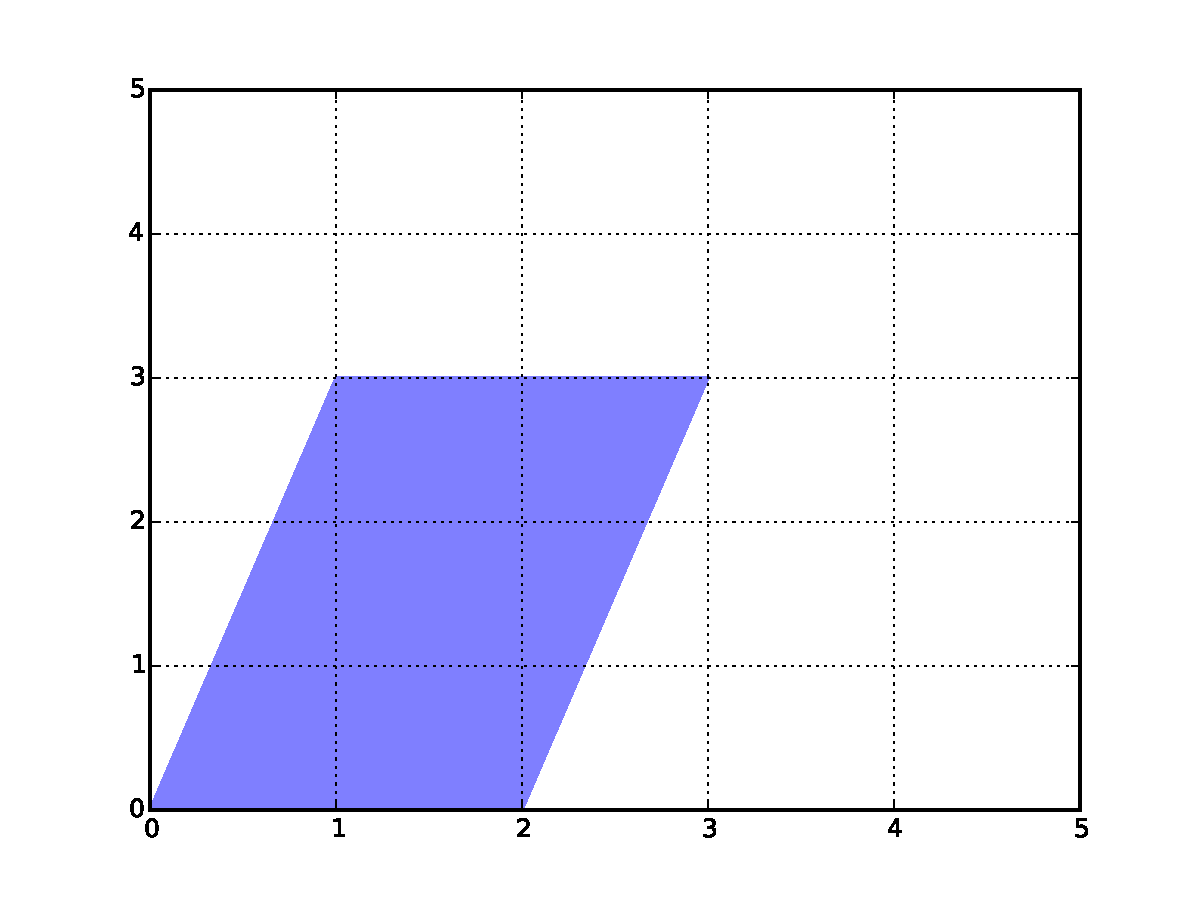
\includegraphics[width=\linewidth]{figs/ex6_1_4.pdf}

\begin{verbatim}
from matplotlib import patches

A= Matrix(2, 2, [2, 1, 0, 3])
A.det() # 6

verts= [(0, 0),
        A.col(0),
        (sum(A.row(0)), sum(A.row(1))),
        A.col(1)]

parall= patches.Polygon(verts, color= 'b', alpha= 0.5)
fig = plt.figure()
ax = fig.add_subplot(1, 1, 1)
ax.add_patch(parall)
ax.set_xlim((0, 5))
ax.set_ylim((0, 5))
plt.grid()
plt.draw()
fig.savefig('figs/ex6_1_4.pdf')
plt.close()
\end{verbatim}

Note that a negative determinant means that area is rotated.

\begin{verbatim}
A1= Matrix(2,2, [1, 2, 3, 0])
A1.det() # -6
\end{verbatim}

Similarly, the determinant of a 3x3 matrix is the volume of the parallelepid described
by the matrix coordinates.

\subsubsection{Exercise 6.1.5}
%-----------------------------

Determine whether the following system has a unique solution

$$
\left [
2 x + 3 y = -2, \quad
5 x - 2 y = 14
\right ]
$$

The system can be re-written in matrix form as

$$
\mathbf{Ax= b} \quad
\left[\begin{matrix}
2 x + 3 y\\5 x - 2 y
\end{matrix}\right] = \left[\begin{matrix}-2\\14\end{matrix}\right]
$$

The determinant of \textbf{A} is $det(\mathbf{A})= -19 \neq 0$, so the system has
a unique solution for $x= 2, y= -2$

\begin{verbatim}
eq1= Eq(2*x + 3*y, -2)
eq2= Eq(5*x - 2*y, 14)
sols= solve([eq1, eq2])

# Can be re-written as 
A= Matrix(2, 2, [2, +3, 5, -2])
det(A) != 0 # True -> Unique solution
b= Matrix([-2, 14])
X= Matrix([x, y])
axb= Eq(A*X, b)
solve(axb) # Same as above
\end{verbatim}

Note that a unique solution is found for any values of the vector \textbf{b}, the
right hand side of the equations or responses. What decides whether the system has
a unique solution are the coefficients in the matrix \textbf{A}, \emph{i.e.} the
left hand side of the equation or predictors. For example:

\begin{verbatim}
X= Matrix([x, y])
A= Matrix(2, 2, [2, +3, 5, -2])
b1= Matrix([-2, 14])
b2= Matrix([7, 5])
b3= Matrix([pi, pi])

for b in [b1, b2, b3]:
    print solve(Eq(A*X, b))
# {x: 2, y: -2}
# {x: 29/19, y: 25/19}
# {x: 5*pi/19, y: 3*pi/19}
\end{verbatim}

\subsection{Determinant of other matrices}
% ========================================

\subsubsection{Exercise 6.2.2}
%-----------------------------

Show that $det(\left[\begin{matrix}
\mathbf{i} & \mathbf{j} & \mathbf{k} \\
7 & 3 & -2\\
4 & 2 & 7
\end{matrix}\right]) =
25 \mathbf{i} - 57 \mathbf{j} + 2 \mathbf{k}$

\begin{verbatim}
i,j,k= symbols('i j k')
M= Matrix(3, 3, [i, j, k, 7, 3, -2, 4, 2, 7])
M.det() #
\end{verbatim}

\subsubsection{Exercise 6.2.3}
%-----------------------------

find $x$ so that
$$
det(\left[\begin{matrix}1 & 0 & -3\\5 & x & -7\\3 & 9 & x - 1\end{matrix}\right]) = 0
$$

We have $det(\mathbf{M}) = x^{2} + 8 x - 72$ , so to have $x^{2} + 8 x - 72 = 0$
we need $x = -4 + 2 \sqrt{22}, \quad x= - 2 \sqrt{22} - 4$. As shown by substituting
these solutions in \textbf{M} and calculating the determinant.

\begin{verbatim}
M= Matrix([[1, 0, -3],
           [5, x, -7],
           [3, 9, x-1]])

detm= det(M)
eq= Eq(detm, 0)
sols= solve(eq)
det(M.subs(x, sols[0])) == 0 # True
det(M.subs(x, sols[1])) == 0 # True
\end{verbatim}

\subsubsection{Exercise 6.2.4}
%-----------------------------


Find the \textbf{cofactor matrix} \textbf{C} of $
\mathbf{A}= \left[\begin{matrix}1 & 0 & 5\\-2 & 3 & 7\\6 & -1 & 0\end{matrix}\right]
$

Cofactor matrix:

$$
\mathbf{C}= \left[\begin{matrix}7 & 42 & -16\\-5 & -30 & 1\\-15 & -17 & 3\end{matrix}\right]
$$

The cofactor matrix is used to calculate the \textbf{inverse} of matrix.

\begin{verbatim}
A= Matrix([[1, 0, 5],
           [-2, 3, 7],
           [6, -1, 0]])
C= A.cofactorMatrix()
\end{verbatim}

Maybe useful to note:

$$
\mathbf{A} = \left[\begin{matrix}x_{1} & x_{2}\\x_{3} & x_{4}\end{matrix}\right] \quad
\mathbf{C_A}= \left[\begin{matrix}x_{4} & - x_{3}\\- x_{2} & x_{1}\end{matrix}\right]
$$

and

$$
\mathbf{A} =  \left[\begin{matrix}x_{1} & x_{2} & x_{3}\\x_{4} & x_{5} & x_{6}\\x_{7} & x_{8} & x_{9}\end{matrix}\right]
\mathbf{C_A}= \left[\begin{matrix}
x_{5} x_{9} - x_{6} x_{8} & - x_{4} x_{9} + x_{6} x_{7} & x_{4} x_{8} - x_{5} x_{7}\\
- x_{2} x_{9} + x_{3} x_{8} & x_{1} x_{9} - x_{3} x_{7} & - x_{1} x_{8} + x_{2} x_{7}\\
x_{2} x_{6} - x_{3} x_{5} & - x_{1} x_{6} + x_{3} x_{4} & x_{1} x_{5} - x_{2} x_{4}
\end{matrix}\right]
$$

\begin{verbatim}
x1,x2,x3,x4,x5,x6,x7,x8,x9= symbols('x1:10')

A= Matrix(2,2,[x1, x2, x3, x4])
A.cofactorMatrix()

A= Matrix(3,3,[x1,x2x,x3,x4,x5,x6,x7,x8,x9])
A.cofactorMatrix()
\end{verbatim}

\subsubsection{Exercise 6.2.5}
%-----------------------------

The inverse of \textbf{A} is:

$$
\mathbf{A}^{-1} = \frac{1}{det(\mathbf{A})} adj(\mathbf{A})
$$

where the \emph{adjoint} of \textbf{A} is the transpose of the cofactor matrix of \textbf{A}:
$adj(\mathbf{A}) = \mathbf{C}^T$

\begin{verbatim}
def inv(A):
    C= A.cofactorMatrix()
    adj= C.transpose()
    inva= (1 / det(A)) * adj
    return inva
\end{verbatim}

Find the inverse of the following matrices.

\begin{verbatim}
A= Matrix(2, 2, [9, 2, 13, 3])
inv(A) # checked against A.inv()

D= Matrix(3, 3, [3, -5, 3,
                 2, 1, -7,
                 -10, 4, 5])
inv(D)
\end{verbatim}

\subsubsection{Exercise 6.2.12}
%-----------------------------

Find the values of $k$ for which the matrix
$\mathbf{A} = \left[\begin{matrix}k & 1 & 2\\0 & k & 2\\5 & -5 & k\end{matrix}\right]$
is invertible. Since inversion requires $det(\mathbf{A}) \neq 0$, we need to get
the determinant of \textbf{A} and
solve it for $k$. Values of $k$ that are not solutions of $det(\mathbf{A}) = 0$ make
\textbf{A} invertible.

$det(\mathbf{A}) = k^3 + 10$ solved for $k$ in
$\left [ - \sqrt[3]{10}, \quad
\frac{\sqrt[3]{10}}{2} - \frac{\sqrt{3} i}{2} \sqrt[3]{10}, \quad
\frac{\sqrt[3]{10}}{2} + \frac{\sqrt{3} i}{2} \sqrt[3]{10}\right ]$

\begin{verbatim}
A= Matrix(3, 3, [k, 1, 2,
                 0, k, 2,
                 5, -5, k])

sols= solve(Eq(A.det(), 0))

## Check A is not invertible for k in sols:
A.subs(k, sols[0]).inv()  ## ValueError: Matrix det == 0; not invertible.
A.subs(k, sols[1]).inv()  ## ValueError: Matrix det == 0; not invertible.
A.subs(k, sols[2]).inv()  ## ValueError: Matrix det == 0; not invertible.

## Check it is invertible for other values of k
A.subs(k, 0).inv()
A.subs(k, sols[0]+1).inv()
A.subs(k, sols[2]+1).inv()
\end{verbatim}


\subsection{Properties of determinants}
% =====================================

As noted above, calculating the determinant of large matrices can take ages. However,
the determinant of diagonal and triangular matrices are very easy to compute:
Just multiply the entries along the leading diagonal. This means that if a matrix can be
rearranged in one or more triangular matrices, by means of row operations and decomposition,
than the calculation of the determiant is much simpler.

\subsubsection{Exercise 6.3.1}
%-----------------------------

Find the determinant of $\mathbf{A}= \left[\begin{matrix}1 & 0 & 0\\0 & -10 & 0\\0 & 0 & 1\end{matrix}\right]$.

The matrix is diagonal: Multiply the entries along the leading diagonal
$det(\mathbf{A}) = (1) (-10) (1)= -10$

\begin{verbatim}
def diagprod(A):
    dp= 1
    for i in range(A.rows):
        dp= dp*A[i, i]
    return dp
    
A= Matrix(3, 3, [1, 0, 0,
                 0, -10, 0,
                 0, 0, 1])
diagprod(A) # -10
# Cheack against
diagprod(A) - A.det() == 0 # True
\end{verbatim}

For $\mathbf{B}= \left[\begin{matrix}1 & 0 & 0\\0 & 0 & 1\\0 & 1 & 0\end{matrix}\right]$

The matrix is not diagonal or triangular as such but it can be made diagonal by
swapping rows.

\begin{verbatim}
B= Matrix(3, 3, [1, 0, 0, 0, 0, 1, 0, 1, 0])
\end{verbatim}

\subsection{LU factorization}
% ===========================

Lower-Upper (LU) factorization decomposes a square matrix in an upper and lower
triangular matrix. After this decomposition the computation of the determinant is
much faster. LU decomposition can also be used as a fast way to solve linear systems.
Computer systems use LU to solve linear systems.

The general procedure to obtain the \textbf{L} and \textbf{U} matrices for a matrix 
\textbf{M} is
\begin{enumerate}
\item Apply row operations $1, 2, \dots, n$ to \textbf{M} until you obtain the \textbf{U} matrix.
\item Now start from the identity matrix \textbf{I}. Apply to \textbf{I} the same row
operations in \emph{reverse} order $n, \dots, 2, 1$ and you get the \textbf{L} matrix.
\end{enumerate}

To solve the system $\mathbf{Ax= b}$ consider the equivalence $\mathbf{Ax = (LU)x = L(Ux) = b}$.
Set $\mathbf{Ux = y}$ and compute \textbf{y}. Now substitute \textbf{y} to
\textbf{Ux} to obtain $\mathbf{Ly = b}$, solve it and you have the solution to the
original system $\mathbf{Ax = b}$. The \textbf{LU} route is much faster than solving
$\mathbf{Ax = b}$ directly since we deal with trangular matrices. 

Home made python code for solving $\mathbf{Ax = b}$ via \textbf{LU} decomposition:

\begin{verbatim}
def LUsolve(A, b):
    x= symbols('x1:%s' %(b.rows+1))
    x= Matrix(b.rows, 1, x)
    Ax_b= Eq(A*x, b)               # Original system Ax = b
    L, U= A.LUdecomposition()[0:2] # Get U & L triang matrices from A
    LUx_b= Eq(L*U*x, b)            # Decompose Ax = b -> (LU)x = b
    assert(LUx_b - Ax_b == 0)      # Check transformation works
    y= U*x                         # Compute Ux = y and use y in place of Ux
    Ly_b= Eq(L*y, b)               #
    assert(Ly_b - Ax_b == 0)       # Check transformation works
    sols= solve(Ly_b, x)           # Solve Ly =b
    return sols
\end{verbatim}

In addition, \textbf{LU} decomposition is useful to find the inverse of a matrix:

$$
\mathbf{A^{-1} = (LU)^{-1} = U^{-1}L^{-1}}
$$

\subsubsection{Exercise 6.4.1}
%-----------------------------

Solve the following linear systems using \textbf{LU} factorization

$$
\mathbf{Ax = b}; \quad
\mathbf{A}= \left[\begin{matrix}1 & 2 & 2\\3 & -3 & -2\\4 & -1 & -5\end{matrix}\right]; \quad
\mathbf{b}= \left[\begin{matrix}5\\0\\-10\end{matrix}\right]
$$

The solution is for $\left \{ x_{1} : 1, \quad x_{2} : -1, \quad x_{3} : 3\right \}$
and it is (obvioulsy) the same whether we use the home made LU solver or
\sympy built in. In fact \sympy probably uses LU decomposition.

\begin{verbatim}
x1, x2, x3= symbols('x1:4')
A= Matrix(3, 3, [1, 2, 2, 3, -3, -2, 4, -1, -5])
b= Matrix(3, 1, [5, 0, -10])
x= Matrix(3, 1, [x1, x2, x3])

sols= LUsolve(A, b) # {x1: 1, x2: -1, x3: 3}

# Check against sympy
axb= Eq(A*x, b)
ssym= solve(axb, x)
for _x in x:
    assert(sols[_x] == ssym[_x])
\end{verbatim}

\subsubsection{Exercise 6.4.2}
%-----------------------------

Same as above solve the linear system $\mathbf{Ax = b}$ for
$\mathbf{A}= \left[\begin{matrix}1 & 2 & 3 & 4\\17 & 22 & 27 & 8\\77 & 44 & 47 & -494\\-10 & 1 & 7 & 63\end{matrix}\right]; \quad
\mathbf{b}= \left[\begin{matrix}-10\\22\\2106\\-243\end{matrix}\right]$

Solved for $\left \{ x_{1} : 1, \quad x_{2} : -2, \quad x_{3} : 3, \quad x_{4} : -4\right \}$.

\begin{verbatim}
A= Matrix([[1, 2, 3, 4],
           [17, 22, 27, 8],
           [77, 44, 47, -494],
           [-10, 1, 7, 63]])
b= Matrix(4, 1, [-10, 22, 2106, -243])

sols= LUsolve(A, b)
\end{verbatim}

\subsubsection{Exercise 6.4.5}
%-----------------------------

Find the inverse of $\mathbf{A}= \left[\begin{matrix}1 & 2 & 3\\3 & 7 & 14\\4 & 13 & 38\end{matrix}\right]$

\begin{verbatim}
A= Matrix(3, 3, [1,2,3, 3,7,14, 4,13,38])
L, U, _= A.LUdecomposition()
Ainv= U.inv() * L.inv()
assert(Ainv == A.inv())

## Note that U^-1 * L^-1 != L^-1 * U^-1
L.inv() * U.inv()
\end{verbatim}